\chapter{Eztabaida.}

\section{Eguzki-sistemaren integraziorako egungo metodoak.}


Tesiaren sarreran azaldu genuenez, gure helburua eguzki-sistemaren epe luzeko eta doitasun handiko inplementazio eraginkorra proposatzea da. Atal honetako ekarpena azaldu aurretik, egungo eguzki-sistemaren simulazioen errepasoa aztertzea interesgarria dela iruditzen zaigu. Bi eratako simulazioak aztertuko ditugu: efemerideak, eguzki-sistemaren eredu konplexuak integratzen dituzte eta integrazio tarte "motzak" dira; Laskar-ek eta bere taldeak, paleoklimatologi ikerketentzako egindako simulazio luzeak.  

\subsection{Efemerideak.}

Konputagailuen aurreko garaian, efemerideak teoria analitikoetan oinarritutako serie funtzioen bidez kalkulatzen ziren. Soluzio hauetan, Fourier-en serie trigonometriko luzeen ebaluazioa egin behar zen. $1960$ hamarkadan, eguzki-sistemaren ezagutza hobetu zenean (espazio bidaiak eta behatoki astronomikoen aurrerapenak medio), serie oso luzeak kalkulatu behar zituzten, eta zenbakizko integrazioen bidezko soluzioak eraginkorragoak bilakatu ziren \cite{Kaplan2015}.   
   
Eguzki-sistemaren gorputzen efemeride modernoak, mugimenduaren ekuazio diferentzialen zenbakizko integrazioaren bidez kalkulatzen dira. Integrazioaren hasierako balioak eta ereduaren parametroak, sateliteen bidez jasotako datuei egokitzen zaizkie.

Efemerideak, \emph{Chebyshev} polinomio moduan adierazten dira. Integrazio tarteak, $2.000.$ urte inguruko ehunka urtekoak izaten dira. Zenbakizko integrazio hauetan, biribiltze errorea gai garrantzitsua da. $128$-biteko aritmetika erabiltzeko aukera oso garestia delako bere erabilera baztertzen da eta $64$-bit doitasuneko aritmetika hobetzeko teknika konputazionalki merkeak aplikatzen dira. 

Efemerideetarako, eguzki-sistemaren eredu konplexua aplikatzen da. Gorputz nagusien arteko indar grabitazionalez gain, erlatibitate efektua, asteroideek eragindako grabitazio indarrak, gorputzen formen eragina eta beste hainbat indar ez grabitazionalak kontutan hartzen dituzte. Mugimenduaren ekuazio diferentzialak hauek dira \cite{Feinga2015},      
      \begin{equation*}
      \ddot{x}_{Planet}= \sum_{A \neq B} \mu_B \frac{r_{AB}}{\|r_{AB}\|^3}+\ddot{x}_{GR} (\beta,\gamma,c^{-4})+ \ddot{x}_{AST,300}+ \ddot{x}_{J_2}.
      \end{equation*}
      
      \begin{itemize}
      \item $8$ planetak, ilargia, Pluton eta 300 asteroide.
      \item GR: erlatibitate efektua (Einstein-Imfeld-Hoffmann, $c^{-4}$ PPN hurbilketa).
      \item $J_2$: eguzkia esferikoa ez izatearen eragina. 
      \item Urrats luzera, $h=0.055$ egunekoa da.
      \end{itemize}   

\subsubsection*{Erlatibitate efektua.}
Eguzkiaren erlatibitate efektua kontutan hartzen duten ekuazio diferentzialak azalduko ditugu.

\begin{equation}
\dot{q_i}=v_i, \  i=0,1,\dots N
\end{equation}

\begin{multline} 
\dot{v_i}= \sum_{j=0,j \neq i}^{N} \frac{Gm_j}{\|q_j-q_i\|^3} (q_j-q_i)
           \bigg(1- \frac{2(\beta+\gamma)}{c^2} \sum\limits_{k=0, k \neq i}^{N} \frac{Gm_k}{\|q_k-q_i\|} 
                  - \frac{2\beta-1}{c^2}        \sum\limits_{k=0, k \neq j}^{N} \frac{Gm_k}{\|q_k-q_j\|} \\
                  + \gamma \big(\frac{v_i}{c}\big)^2 + (1+\gamma) \big(\frac{v_j}{c} \big)^2 
                  - \frac{2(1+\gamma)}{c^2} v_i \ v_j \\
                  - \frac{3}{2c^2} \big(\frac{(q_i-q_j) v_j}{\|q_j-q_i\|} \big)^2+                  
                  \frac{1}{2c^2}(q_j-q_i) \dot{v_i} \bigg) \\
           + \frac{1}{c^2} \sum_{j=0,j \neq i}^{N} \frac{Gm_j}{\|q_j-q_i\|^3} 
             ((q_i-q_l) ((2+2\gamma)v_i-(1+2\gamma)v_j)) (v_i-v_j) \\
           + \frac{3+4\gamma}{2c^2} \sum_{j=0,j \neq i}^{N} \frac{Gm_j \dot{v_j}}{\|q_j-q_i\|}                                      
\end{multline}

\begin{table}[h]
\caption{Konstanteak}
\label{tab:1}       % Give a unique label
\centering
\begin{tabular}{l l l }
\hline
  c             &  $299792.458$ km/s           & Argiaren abiadura  \\
%\hline
  au            &  $149597870.700$ km          & Unitate Astronomikoa  \\
%\hline 	       
$\beta$          & $1.0$                       & PPN parametroa     \\
%\hline 
$\gamma$         & $1.0$                       & PPN parametroa     \\
\hline
\end{tabular}
\end{table}

\subsubsection*{Asteriodeak.}
Asteroideek, bereziki Marte planetaren mugimenduarengan eragina dute (\ref{fig:asteroideak} irudia) eta kontutan hartzekoak, barne planeten mugimenduaren doitasun handiko emaitzak behar ditugunean . Bost asteroide nagusiren masak (Ceres, Pallas, Vesta, Iris eta Bamberga) Merkurio eta Pluton planeten mailakoak direnez, integrazioetan gehitzen dira. Beste asteroide txikien talde handia, estimazioen bidez simulatzen dira.

\begin{figure} [h]
\centerline{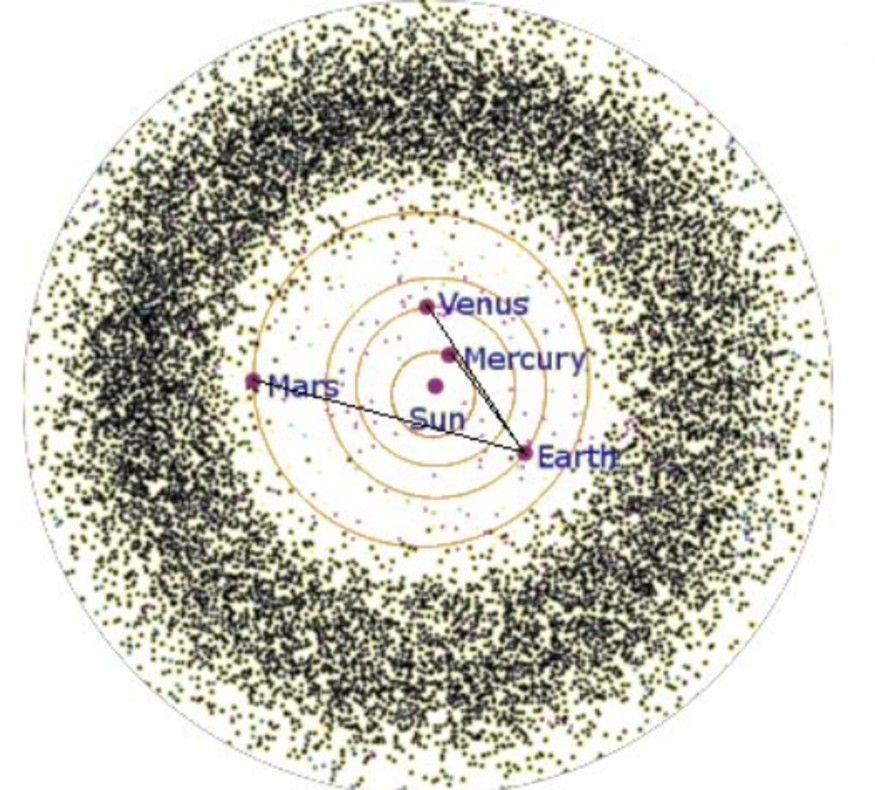
\includegraphics [width=6cm, height=4cm] {Asteroideak}}
\caption{Asteroideak.}
\label{fig:asteroideak}
\end{figure} 

  
\subsubsection*{Hiru efemerideak.}

Gaur-egun, eguzki-sistemaren planeten hiru efemeride kalkulatzen dira.
\begin{enumerate}
\item Jet Propulsion Laboratory (\emph{EEBB}) \emph{NASA}-ko erakundeak DE (Development Ephemerides) izeneko efemerideak.

      $1984$.urtean kalkulatu zen lehen efemeridea (DE-200) eta $2.014$.urteko da \emph{DE-430} \cite{Folkner2014} publikatutako azken efemeridea. Kalkulatutako integrazio tartea, ($1550-2650$) izan da.

      Zenbakizko integrazio metodoa: urrats luzera eta  ordena aldakorreko \emph{Multistep Adams} metodoa, \cite{Krogh1997} \emph{DIVA}/\emph{QIVA}. \emph{QIVA} doitasun laukoitzeko ($128$-bit) bertsioari deitzen zaio: mugimenduaren ekuazioen Newton zatia, doitasun laukoitzean kalkulatzen da eta ekuazioaren gainontzeko zatia, doitasun bikoitzean.

\item Institut de Méchanique Céleste et de Calcul des Ephémérides (IMCCE,Paris Observatory) INPOP (Intégrateur Númerique Planétaire de l'Observatoire de Paris) izeneko efemerideak.
      
      $2.000$.arte, teori analitikoetan oinarritutako efemerideak garatu zituzten. $2.003$.urtean kalkulatu zuten lehen zenbakizko integrazio bidezko efemeridea eta \emph{INPOP13c} ($2.014$) \cite{Fienga2008} publikatutako azkena da.
           
	  Zenbakizko integrazio metodoa: $12$ ordeneko \emph{Adams-Cowell} metodoa da eta urrats finkoa aplikatzen du.
	  
	  Doitasuna: C lengoaian inplementatuta dago eta \emph{Intel} makinetako $80$-biteko doitasuna erabiltzen du. Era berean, modu merkean doitasun handitzeko, doitasun laukoitza simulatuz urrats zuzentzaile (corrector step) bat aplikatzen zaio \cite{Fienga2008}.  
	  
  
\item Institute of Applied Astronomy (\emph{IAA}, St. Petersburg), EPM (Ephemerides Planets-Moon) izeneko efemerideak.
      
      $1.980$.urtetik aurrera, zenbakizko integrazioen bidezko efemerideak kalkulatu dituzte eta  \emph{EPM2.013} ($2.014$) \cite{Pitjeva2014} publikatutako azken efemeridea da.
      
      Zenbakizko integrazio metodoa. \emph{Everhart} izeneko \emph{IRK} metodoa (Gauss-Radau) da. $23$ ordeneko metodoa eta urrats luzera finkoa aplikatzen du.
            
      Doitasuna. Inplementazioak (software package ERA), \emph{Intel} makinetako $80$-biteko doitasuna erabiltzen du.
      
\end{enumerate}


(\ref{fig:668}) taulan, planeten efemerideen doitasunaren eboluzioa ikus daiteke. Hiru efemerideak antzeko doitasuna azaltzen dutela gehitu beharra dago. 
\begin{figure} [h]
\centerline{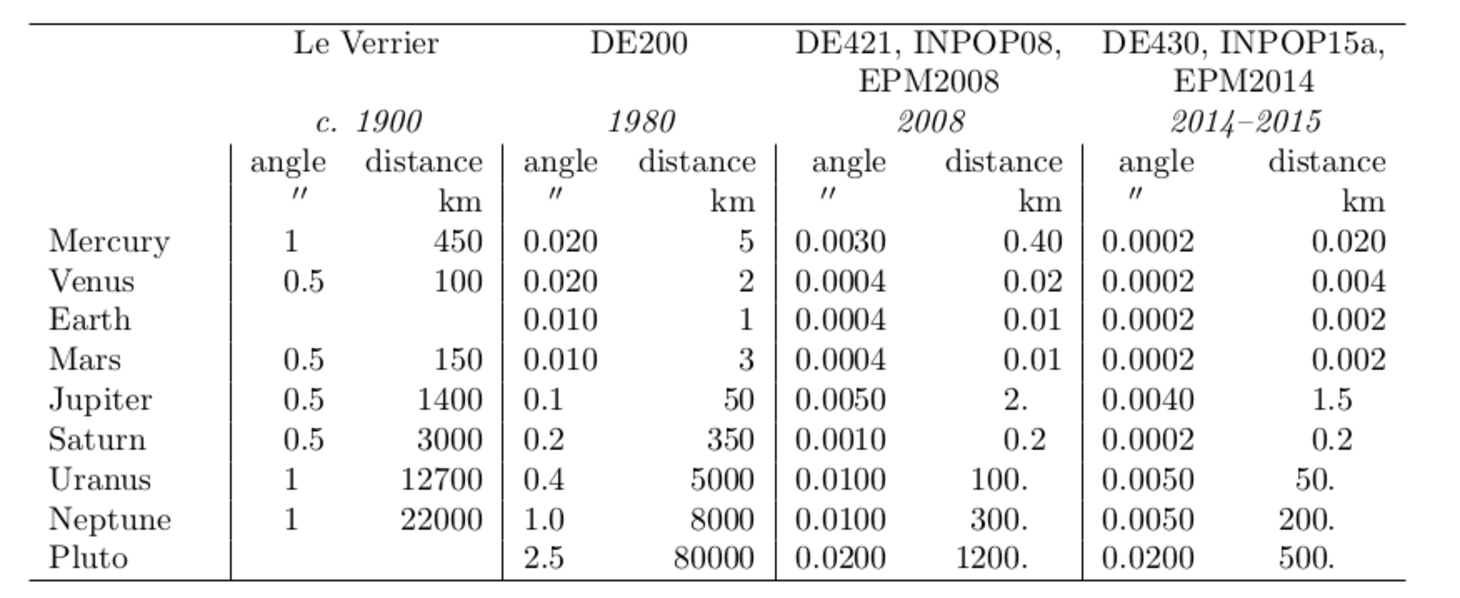
\includegraphics [width=10cm, height=6cm] {Efemerideak}}
\caption{Efemerideen doitasunaren eboluzioa.}
\label{fig:668}
\end{figure} 

\subsection{Eguzki-sistemaren integrazio luzeak.}


A.Morbidellik \cite{Morbidelli2002} eguzki-sistemaren zenbakizko integrazioen algoritmoen garapenaren azterketan, garai hauek bereizten ditu:
\begin{enumerate}

\item Garai klasikoa.

$90$. hamarkada hasiera arte, urrats luzera aldakorreko integratzaileak erabiltzen dira: Runge-Kutta (Dormand et al. $1987$), Bulirsch and Stoer ($1966$), Radau (Everharht, $1985$), eta Störmer ($1990$). Garai honetan integrazio tarteak, $10^4-10^6$ urte artekoak dira.  

\item Garai sinplektikoa.

Wisdom eta Holman-en \cite[1991]{Sussman1992} lanarekin, eguzki-sistemaren azterketarako integratzaile sinpletikoen erabilera zabaldu zen. Garai honetan, ($10^8-10^9$) urte arteko eguzki-sistemaren integrazioak egin ziren.  

\item Garai estatistikoa.

Planeten eta gorputz txikien (asteroide, meteoritoak) arteko kolisio gertuko egoerak kalkulatzen dituzten algoritmoak garatu ziren. Inplementazio berri hauetan, milaka gorputzen integrazio azkarra egin daiteke. Horrela, asteroide eta meteoritoen orbiten distribuzio azterketa estatistikoak egin ziren.

\item Planeten sorrera garaiko azterketak.

Eguzki-sistemaren sorrerari buruzko simulazioak nagusituko dira; masa handiko gorputzen arteko kolisio gertuko egoerak gertatzen diren integrazioak dira. 
 
\end{enumerate}

Eguzki-sistemaren integrazioetarako nagusiki, bi integratzaile famili aplikatzen da: 
\begin{enumerate}
\item Integratzaile simetrikoak.

Metodo simetrikoen artean nagusiena, 4 ordeneko \emph{Hermite} \cite{Aarseth2008} integratzailea da.
Urrats luzera tamaina aldakorreko integratzaile da, modu errazean inplementatu daiteke.  Hermite integratzailea konputazionalki garestia da eta bereziki, gorputz kopuru handia dituzten eta kolisio gertuko egoerak maiz gertatzen diren problemetan (eguzki-sistemaren sorrera, \dots) aplikatzen da.  

\item Sinplektikoak.

Gaur-egun, eguzki-sistemaren epe luzeko integrazioetarako, integratzaile sinplektikoak nagusitu dira. 

\end{enumerate}

Eguzki-sistemaren integrazio luzeei buruzko beste errebizio dokumentu interesgarri hauek aholkatu nahiko genituzke: \cite{Kholshevnikov2007} (Kholshevnikov2007, $2.007$), \cite{Brumberg2013} (Brumberg, $2.013$) eta  \cite{Ito2007} (Ito eta Tanikawa, $2.007$).  
 


\subsubsection*{Eguzki-sistemari egokitutako integratzaile sinplektikoak.}

Wisdom-ek eta Holman-ek \cite[1991]{Sussman1992}, eguzki-sistemaren epe luzeko simulazioetarako integratzaile  sinplektikoak (\emph{WH}) arrakasta izan zuen. Eguzki-sistema, mugimendu perturbatua duen sistema dinamikoa da eta ezaugarri honi egokitutako integratzaile eraginkorra garatu zuten. N-gorputzen problemaren Hamiltondarra,  Jacobi koordenatuak  aplikatuz, bi zatitan banatu zuten,
\begin{equation*}
H(q,p)=H_K(p)+H_I(q) \ \ \ , \ \ H_K\gg H_I,
\end{equation*}
non $H_K$, Hamiltondar Kepleriarra (planeten eguzkiarekiko mugimendu kleperiarra) eta $H_I$, interakzioen Hamiltondarra (planeten arteko grabitazio interakzioak) diren. Integrazioaren urrats bakoitzean , Hamiltondar bakoitzaren soluzioa tartekatuz, problema osoaren ebazpena kalkulatzen da.  

\emph{WH} integratzailea, ondorengo metodoen aurrekaria kontsideratu bada ere, bere aplikagarritasuna mugatua da. Batetik, izar anitzeko planeten sistemak edo planeta-ilargiak sistemak integratzeko ez da egokia. Bestetik, \emph{WH} metodo sinplektikoa denez urrats luzera finkoa aplikatu behar da eta gorputzen arteko kolisio gertuko egoerak dituzten problemak, modu eraginkorrean integratzeko eragozpen bat da. Arazo hauek gainditzeko, urteetan zehar algoritmo honen aldaerak proposatu dira eta jarraian, nagusienak aipatuko ditugu. 

Levinson eta Duncan-ek \cite[1994]{Levison1994}, \emph{WH} inplementazioa, integratzaile ez sinplektiko batekin konbinatu zuten kolisio egoeren kalkulua hobetzeko. \emph{SWIFT} paketean, \emph{RMVS3} izeneko integratzailea inplementatu zuten. Duncan, Levinson eta Lee-k \cite[1998]{Duncan1998}, koordenatu Heliozentrikoak erabiliz, Hamiltondarra beste modu honetan banatu zuten,  
\begin{equation*}
H(q,p)=H_K(p)+H_C(p)+H_I(q)
\end{equation*}
eta kolisiotik gertuko egoerei, urratsa luzera txikituz aurre egin zioten. Inplementazio honek, \emph{SYMBA} izena du. Chambers-ek \cite{Chambers1999} koordenatu Heliozentrikoetan oinarritu zen eta kolisio egoerak gertatzen diren uneetan, beste integratzaile  (Bulirsch-Stoer metodoa) batekin konbinatuz integratzen du. Inplementazio honek, \emph{MERCURY} izena du. Levinson eta Duncan-ek ($2000$), aurreko inplementazioaren arazo batzuk konponduz, \emph{Modified SYMBA} izeneko garapen berria burutu zuten.
Kvaerno eta Leimkuhler \cite{Kvaerno2000} eta beste autore batzuk ere, antzeko ideiak landu dituzte.

Wisdom eta Holmanek proposatutko Hamiltondarraren banaketa, \emph{Leapfrog} metodoaren bidez integratzen da eta beraz, 2 ordeneko da. Orden altuagoko ($p>2$) metodoak definitzeko, koefiziente negatiboak erabili behar dira \cite{Yoshida1993,Laskar2001} eta ez dira interesgarriak, \emph{Leapfrog} metodoa hauek baino eraginkorragoa baita. 

\paragraph*{Adibidea.}
Yoshidaren $p=4$ ordenako metodoa. $\phi_h$ oinarrizko metodoa \emph{Leapfrog} izanik, metodoaren konposaketari dagokion 4 ordeneko konposizio metodoa, era honetan definitzen da,
\begin{equation*}
\Psi_h=\phi_{\gamma_1 h} \circ \phi_{\gamma_0 h} \circ \phi_{\gamma_{1 h}},
\end{equation*}  
non  $\gamma_0=-2^{1/3}/(2-2^{1/3})$ eta $\gamma_1=1/(2-2^{1/3})$.

Beranduago, McLachlan-ek \cite[1995]{McLachlan1995}, Laskar-ek eta Robutel-ek \cite[2001]{Laskar2001} koefiziente negatiboen arazoa gainditu zuten eta ordena altuko Splitting eskemak aurkitu zituzten. Berriki, Blanes et al \cite[2012]{Blanes2013} ordena altuko Splitting eskema berriak eta eraginkorrak aurkitu ditu. 

Azken aldian, Hernandez eta Bertschinger-ek \cite[2015]{Hernandez2015} N-gorputzen problema grabitazional eta kolisiodunetarako 2 ordeneko integratzaile sinplektiko berri bat proposatu dute. Hernandez eta Bertschinger-ek \cite{Hernandez2015} koordenatu kartesiarretan oinarrituz, N-gorputzen problema 2-gorputzen problemetan banatzen dute eta honako Hamiltondarraren banaketa proposatzen dute,
\begin{align}
\begin{split}
&H=T+V, \\
&H=T+ \sum_{i} \sum_{i>j} V_{ij}, \\
&H=T+ \sum_{i} \sum_{i>j} (K_{ij}-T{ij})
\end{split}
\end{align}

\section{Jorratutako bideak.}

\subsection*{Atalen hasieraketa.}

Puntu-finkoaren iterazioan, atalen hasieraketa teknika ezberdinak ikertu ditugu. 
\begin{enumerate}
\item Metodo esplizituak.

Euler-en eta Euler-hobetuaren metodoak aztertu ditugu.

\item Kepler fluxua.

Eguzki-sistema, perturbatutako sistema Kepleriarra dela jakinda, atalak Kepler fluxuaren bidez hasieratu daitezke.

\item Interpolazio polinomioak.

Aurreko urratseko ataletako informazioa erabiliz, urrats berriaren atalen hasieraketa lortzen dugu. Problema zurruna ez denean interesgarria da. 

Bide honetatik, teknika aurreratuagoak ere aztertu ditugu (maila txikiko polinomioen bidezko hasieraketak). Era berean, B-Serieak \cite{Chartier2010} teknikan oinarrituz interpolazio koefiziente optimoagoak lortzeko saiakera egin dugu.

\end{enumerate}

\subsection*{Geratze irizpidea.}

\subsubsection*{Norma.}
Lehengo, geratze irizpidea definitzeko norma zalantzan jarri dugu. Hairer-ek, geratze irizpidean aplikatzen duen norma hauxe da,
\begin{equation*}
\Delta Y= \max_{i=1,\dots,s} \|Y_i^{[k]}-Y_i^{[k-1]}\|_{\infty}.
\end{equation*}

Aukera ezberdinak aztertu ondoren, honako norma finkatu genuen, 
\begin{align*}
\Delta Y= \max_{1 \leqslant j \leqslant s} \frac{\max_{1 \leqslant j \leqslant s} |\Delta Y_i^j|}
                                                {(\max_{1 \leqslant j \leqslant s}|Y_i^j|)+\delta},
\end{align*}
non $\delta \approx 10^{-20}$ zero den kasua ekiditeko balio txikia den eta $y=(y^1,\dots,y^d)$.

\subsubsection*{Geratze irizpidea.}


\section{IRK Newton.}

$(I_s \otimes I_d - h \ A \otimes J) \triangle Y = r$ ekuazio sistema modu eraginkorrean askatzeko, inplementazio estandarraren eta gure inplementazioen konplexutasunak konparatuko ditugu.

\subsection*{Inplementazio estandarra.}

Butcher edota Hairer-en inplementazio estandarraren konputazio bi modutan egin daiteke:

\begin{enumerate}
\item Zenbaki konplexuak.

$A$ matrizearen diagonalizazioak balio propio konplexuak ditu, 
\begin{equation*}
P^{-1}AP=\begin{bmatrix}
  \gamma_1 &                &          &                &           &                 \\
           & \bar{\gamma_1} &          &                &           &                 \\
           &                & \gamma_2 &                &           &                 \\
           &                &          & \bar{\gamma_2} &           &                 \\ 
           &                &          &                & \gamma_3   &                 \\
           &                &          &                &            & \bar{\gamma_3} \\  
\end{bmatrix},
\end{equation*}

eta ekuazio-sistema, zenbaki konplexuen aritmetika erabiliz ebatzi daiteke.
\begin{align*}
&(I-h \gamma_j J) \ X = b, \ \ j=1,\dots,3, \\
&(I-h \bar{\gamma}_j J) \ X = \bar{b}. 
\end{align*}

\item Zenbaki errealak.

Zenbaki konplexuekin ez bada lana egin nahi, zenbaki errealeko deskonposaketa baliokidea,
\begin{align*}
&\gamma_j=\alpha_j + i \ \beta_j,\\
&P^{-1}AP=\begin{bmatrix}
\alpha_{1} & -\beta_{1}   &  0            &  0            &  0           &    0       \\
\beta_{1}  & \alpha_{1}   & 0             &  0            &  0           &    0       \\
 0          & 0             & \alpha_{2}  & -\beta_{2}    &  0           &    0       \\
 0          & 0             & \beta_{2}   & \alpha_{2}    &  0           &    0       \\
 0          & 0             &  0          & 0             & \alpha_{3}  & -\beta_{3}  \\
 0          & 0             &  0          & 0             & \beta_{3}   & \alpha_{3}  \\
\end{bmatrix}
\end{align*}

\end{enumerate}

Hairer-en inplementazioan,
\begin{itemize}
\item $s$ bikoitia bada $\rightarrow$ $(2d \times 2d)$ tamainako $[s/2]$  LU deskonposaketa.
\item $s$ bakoitia bada $\rightarrow$ $(2d \times 2d)$ tamainako $(s+1)/2$  LU deskonposaketa.
\end{itemize}

\subsection*{Gure inplementazio berria.}

$\bar{A}$ matrizearen, $\bar{A}=P^{-1}DP$ diagonalizatzen dugu eta $D$ matrizeak, irudikari puruak ditu,
\begin{equation*}
\bar{A}=Q^{-1}RQ, \ \,
R=\begin{bmatrix}
0           & -\gamma_{1}   &            &               &             &           \\
 \gamma_{1} & 0             &            &               &             &           \\
            &               & 0           & -\gamma_{2}  &             &           \\
            &               & \gamma_{2}  & 0              &           &           \\
            &               &             &                & 0            & -\gamma_{3} \\
            &               &             &                & \gamma_{3}   & 0            \\
\end{bmatrix}
\end{equation*}

Gure inplementazioan,
\begin{itemize}
\item $s$ bikoitia bada $\rightarrow$ $(d \times d)$ tamainako $[s/2]+1$  LU deskonposaketa.
\item $s$ bakoitia bada $\rightarrow$ $(d \times d)$ tamainako $(s+1)/2$  LU deskonposaketa.
\end{itemize}

\subsection*{Konplexutasun konparaketa}

Lehenengo eragiketa aljebraikoen konplexutasunak gogoratuko ditugu,
\begin{align*}
&\text{LU deskonposaketa}:  \ \ 2s^3d^3/3+\mathcal{O}(d^2), \\
&\text{Back substitution}:  \ \ 2s^2d^2+\mathcal{O}(d), \\
&\text{inv}: \ \ 2s^3d^3
\end{align*}

Bi inplementazioen konplexutasunen laburpena,
\begin{table}[h!]
\caption[LU deskonposaketak] 
{\small{}}
\label{tab:Olu}       
\centering
{%
\begin{tabular}{ l l l l l } 
 \hline
\\
                 &  \multicolumn{2}{c}{LU}  & \multicolumn{2}{c}{Back Substitution}  \\
 s               & Estandarra  & Berria     &  Estandarra  &              Berria     \\
\\
 \hline
\\
 $2m$            &   $\frac{8m}{3} d^3$                              &  $\frac{2}{3} (2m+1) d^3$ 
                 &   $4m (2d^2)$      &     $(6m+4)d^2$                                             \\
 \\
 $2m+1$          &   $\left(\frac{8m}{3} + \frac{2}{3}\right) d^3$   &  $\left(\frac{4m}{3}+\frac{2}{3}\right) d^3$
                 &   $(8m+2)d^2$      &     $(6m+4)d^2$\\  
 \\  
   \hline
 \end{tabular}}
\end{table}